\section{Actions} \label{sec:actions}
All \src{Dockable}s can be associated with some actions. An action normally appears as some kind of button in the title of a \src{Dockable}, they can however appear at other places as well. There are different types of actions, some may behave like a \src{JButton} others like a \src{JCheckBox}, clients can add new types.

\begin{figure}[h]
\centering
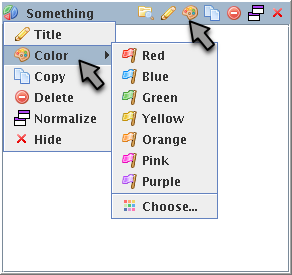
\includegraphics[scale=0.5]{actions/actions}
\caption{A \src{Dockable} with a few \src{DockAction}s in its title and on a popup menu. The action marked by an arrow is the same object just shown in different views.}
\label{fig:actions}
\end{figure}

Actions are represented by the interface \src{DockAction}. Each \src{Dockable} has a list of them represented by a \src{DockActionSource}.

If some component wants to show some actions it firsts asks a \src{Dockable} for its global \src{DockActionSource}. It then asks each \src{DockAction} of that list to create a view that fits to the component. A title will ask for another kind of view than a menu. At any time actions can be added or removed from the \src{DockActionSource} and any component showing actions will react on these events.

\classbox{The interface \src{DockAction} is quite simple. Two methods to install (\src{bind}) and to uninstall (\src{unbind}) the action. One method to create new views (\src{createView}) and one method to trigger an action programatically (\src{trigger}). More useful are the many subclasses and subinterfaces. \src{StandardDockAction} introduces icons, text and tooltip. Five subinterfaces for \src{StandardDockAction} exist and for all of them a default-view is provided.}

\designbox{There are three levels in the design of \src{DockAction} and its subclasses. First there is \src{DockAction} which allows almost any kind of \src{Component} to be used as view. Second there are subinterfaces for the standard tasks, the framework provides views for them. Third are real implementations of the second-level interfaces. Some interfaces are implemented in more than one action for different styles of aplication organization.}

\subsection{Show Actions}
Assuming one has a \src{DockAction} (more about different kind of actions is in the next chapter) how can the framework be advised to show it? 

\subsubsection{List of Actions}
\src{DockAction}s never travel alone in this framework. They always travel with other actions in a \src{DockActionSource}. Actions can be added or removed from \src{DockActionSource}s at any time and modules showing actions will react on this.

Most methods of \src{DockActionSource} can be understood without explanation. The method \src{getLocationHint} is an exception. It returns a  \src{LocationHint} which is used to order several \src{DockActionSources} into a list (and treat them as one big \src{DockActionSource}). Clients which implement an \src{ActionOffer} can also introduce new kind of \src{LocationHint}s.

\classbox{\src{LocationHint}s consists of an \src{Origin} and a \src{Hint}. The hint tells the preferred location in respect to other elements, the origin are used if multiple hints collide. New \src{Hint}s and \src{Origin}s can be written.}

\subsubsection{Source of Actions}
Actions have different sources, each kind of source has a specific purpose.

\begin{itemize}
 \item The \textbf{local action source} is part of every \src{Dockable}. This source is accessed through \src{getLocalActionOffers}. If \src{AbstractDockable} or a subclass like \src{DefaultDockable} is used then \src{setLocalActionOffers} allows to quickly set and exchange the actions. This source of actions should be used for actions that are closely linked with some \src{Dockable}.
 \item \src{ActionGuard}s can add actions to every \src{Dockable}. An \src{ActionGuard} is added to a \src{DockController} through \src{addActionGuard}. Its method \src{react} will be called whenever the actions of a \src{Dockable} are searched. If \src{react} returns \src{true} then the method \src{getSource} is called. This source of actions is intended for general purpose actions and for actions which need a special position in the list of actions (e.g. a close-action needs to be at the very end).
 \item Every \src{DockStation} can add \textbf{direct} and \textbf{indirect action offers} to its children. For this \src{DockStation} has two methods \src{getDirectActionOffers} and \src{getIndirectActionOffers}. \textbf{Direct action offers} are used only for true children, \src{indirect action offers} can be applied to grand-children as well. These sources of actions are intended for actions that are linked to a \src{DockStation}, like the maixmimze-action that can be seen on a \src{SplitDockStation}.
\end{itemize}

Two mechanisms are responsible for collecting all the actions from these different sources and to put them into a list. Clients can adjust these mechanisms even to a point where they no longer collect actions but introduce their own actions.

\begin{itemize}
 \item Every \src{DockController} has at least one \src{ActionOffer}. An \src{ActionOffer} has two methods: \src{interested} tells whether the offer is interested in managing a certain \src{Dockable} and \src{getSource} collects the actions of an interesting \src{Dockable}. The primary function of an \src{ActionOffer} is to order the various sources. It is up to the offer to decide how to actually do the sorting. The default \src{ActionOffer} uses the \src{LocationHint} which is attached to every \src{DockActionSource}.

Clients can use \src{addActionOffer} and \src{setDefaultActionOffer} to change the offers of a \src{DockController}. The public method \src{listOffers} then advises the controller to use one of its offers.

 \item Modules which need a list of actions call \src{getGlobalActionOffers} from \src{Dockable}. This method is the ultimate piece of code which decides what to show. This method can ignore anything else that has been said in this chapter and introduce its very own mechanism to collect actions. 
\end{itemize}

Most \src{Dockable}s will utilize \src{HierarchyDockActionSource} instead of implementing \src{getGlobalActionOffers}. This special source observes the hierarchy of a \src{Dockable} and changes its content automatically. \src{Dockable}s using \src{HierarchyDockActionSource} should \src{bind} the source. They need to call \src{update} if their own local action source is exchanged. 

\warningbox{It is generally a bad idea to write \src{DockActionOffer}s or \src{getGlobalActionOffer} methods which do not just collect actions. There are already mechanisms to introduce \src{DockAction}s and they should suffice for every possible situation.}

\subsection{Standard Actions}
There are a number of standard actions in the framework. Clients can either subclass them or instantiate and add listeners to them. A user would put the actions into six groups:
\begin{description}
 \item[Button] If the user clicks this action then always the same thing happens. The interface \src{ButtonDockAction} collects all the buttonlike actions.
 \item[Checkbox] When triggered it changes some property from \src{true} to \src{false} or from \src{false} to \src{true}. All actions with this behavior implement the interface \src{SelectableDockAction}.
 \item[Radiobutton] Like a group of checkboxes, but only one radiobutton can be selected within that group. Like checkboxes all these actions are represented by \src{SelectableDockAction}. Several radiobuttons can be linked together with the help of a \src{SelectableDockActionGroup}.
 \item[Menu] A menu just contains a list of other \src{DockAction}s. These other actions are normally hidden and only shown if the user wants to see them. Menus are implementing the interface \src{MenuDockAction}.
 \item[Drop-down-button] Like a menu but the last triggered action can be triggered again without opening the menu. The interface \src{DropDownAction} represents these special menus.
 \item[Separator] A separator just is a line, a graphical element to divide a set of actions into subsets. Separators are implemented through the class \src{SeparatorAction}.
\end{description}

\subsubsection{Simple actions}
Simple actions are a set of classes that implement the various action-interfaces. These simple actions do not have any advanced features and should be quite simple to use. An example might be the following code:

\begin{lstlisting}
public class ExampleAction extends SimpleButtonAction{
	public ExampleAction() {
		setText( "Run..." );
		setIcon( new ImageIcon( "example.png" ) );
		setTooltip( "Run the example" );
	}

	@Override
	public void action( Dockable dockable ) {
		System.out.println( "kabum" );
	}
}
\end{lstlisting}

Here the class \src{SimpleButtonAction} is used. The action is subclassed by \src{ExampleAction}. In lines \src{3-5} properties like the icon are set. The subclass overrides the method \src{action} (lines \src{9-11}) which is invoked every time when the user presses the button.

The available simple actions are:
\begin{itemize}
	\item \src{SimpleButtonAction}: For creating buttons. Can either be subclassed (like in the example above) or just instanciated. Clients can add instances of the well known \src{ActionListener}s which will be invoked when the user presses the button. Exaclty like a \src{JButton}.
	\item \src{SimpleSelectableAction.Check} and \src{SimpleSelectableAction.Radio}: \linebreak For creating checkboxes and radiobuttons. Clients can add instances of \linebreak \src{SelectableDockActionListener} to be informed whenever the state of the action changes. A \src{SelectableDockActionGroup} can be used to make sure that only one action out of a set of actions is selected at any time.
	\item \src{SimpleMenuAction}: For creating menus. The method \src{setMenu} takes a \src{DockActionSource} and the content of this source will be shown.
	\item \src{SimpleDropDownAction}: For creating drop down menus. Has methods to get and set the selection, and methods to add or remove actions from the menu.
\end{itemize}

\subsubsection{Group actions}
Group actions are \src{DockAction}s that can be used for many \src{Dockable}s at once even with different properties for each \src{Dockable}. To be more precise, a \linebreak \src{GroupKeyGenerator} will assign a key to each \src{Dockable}. If any view asks the action for a property (like the icon) this key will be used to search the property in a map. All the group actions extend the class \src{GroupedDockAction}.

Let's have a look at an example. The following action behaves like a checkbox. Its unique feature is the text that changes if the selected-state changes.
\begin{lstlisting}
import bibliothek.gui.Dockable;
import bibliothek.gui.dock.action.actions.GroupKeyGenerator;
import bibliothek.gui.dock.action.actions.GroupedSelectableDockAction;

public class ExampleGroupAction extends 
			GroupedSelectableDockAction.Check<Boolean> {
    public ExampleGroupAction(){
        super( new GroupKeyGenerator<Boolean>(){
        	public Boolean generateKey( Dockable dockable ){
        		return dockable.<getSomeProperty()>;
        	}
        });
        setRemoveEmptyGroups( false );
                
        setSelected( Boolean.FALSE, false );
        setSelected( Boolean.TRUE, true );
        
        setText( Boolean.FALSE, "Unselected" );
        setText( Boolean.TRUE, "Selected" );
    }
    
    @Override
    public boolean trigger( Dockable dockable ) {
        setSelected( dockable, !isSelected( dockable ) );
        return true;
    }
    
    @Override
    public void setSelected( Dockable dockable, boolean selected ){
    	dockable.<setSomeProperty( selected )>;
    	setGroup( selected, dockable );
    }    
}
\end{lstlisting}
The constructor (lines \src{7-20}) sets up the action. First the \src{GroupKeyGenerator} is set in lines \src{9-12}. The key is a \src{Boolean} which represents ``some property'' of a \src{Dockable}. The meaning of the property is not important. Through the keys \src{Dockable}s get grouped. When \src{Dockable}s get added and removed a group may become empty. Line \src{13} ensures that the action does not delete the properties of empty groups.

A \src{Boolean} only has two states, both states will be used as key. So there is a ``true'' and a ``false'' group. The selected-state of the action should match the key of the group. In other words: if ``some property'' is \src{true} then the action is selected, if ``some property'' is \src{false} then it is not. Lines \src{15, 16} are responsible for this setting. The same behavior is enforced for the text of the action in lines \src{18, 19}.

The standard behavior of a \src{SelectableDockAction} is to change its selected state as soon as the user triggers the action. If the action is used for many \src{Dockable}s than this behavior would look rather odd. All the actions would change their state and most of them would do so wrongly. By overriding the method \src{trigger} this problem can be prevented (lines \src{23-26}). Instead of changing the selected state of the action, the group of the \src{Dockable} is changed by invoking \src{setSelected} in line \src{24}. Since the two groups have different selection states the user will think that the action changed the state.

By the way: the method \src{setSelected} in lines \src{29-32} needs to be overriden since the default behavior is to change the state of the action, not to change the group of a \src{Dockable}.

\warningbox{Be careful when using group actions: they are complex to handle. In many cases a simple action can replace a group action.}

\designbox{Group actions were introduced for \src{DockStation}s. \src{DockStation}s need to apply the same actions to many \src{Dockable}s. Instead of setting up new actions all the time it was easier to have one action that holds many properties at the same time. }

\classbox{There are only three group actions implemented: 

\begin{itemize}
	\item \src{GroupedButtonDockAction}
	\item \src{GroupedSelectableDockAction.Check}
	\item \src{GroupedSelectableDockAction.Radio}
\end{itemize}}

\subsection{Custom actions}
Clients are free to implement new actions.

\subsubsection{Reuse existing view}
Whenever possible an existing view should be reused. There are 6 kind of views defined in the framework. Each kind of view is represented through an instance of \src{ActionType}, each of them is stored as constant in \src{ActionType} itself. \src{ActionType} has one generic parameter. The view can force an action to implement some interface through that parameter. For example, the kind \src{ActionType.BUTTON} forces an action to implement \src{ButtonDockAction}. Actions can use an \src{ActionType} as key for a factory that is stored in the \src{ActionViewConverter}. 

An example for an action that uses an \src{ActionType} to create its view:
\begin{lstlisting}
public class ExampleButtonAction implements ButtonDockAction{

	public <V> V createView( ViewTarget<V> target,
			ActionViewConverter converter, Dockable dockable ){
	
		return converter.createView( ActionType.BUTTON, this, 
			target, dockable );
	}
	
	public void action( Dockable dockable ){
		[...]
	}
	
	public Icon getIcon( Dockable dockable ){
		return [...];
	}
	
	[...]
}
\end{lstlisting}
Really important are the lines \src{3-8}: these lines are all that is necessary to create different button-views for different environments (menu, title). The \src{ActionViewConverter} does all the work, it just has to be called with the correct parameters.

The interface \src{ButtonDockAction} declares other methods like \src{getIcon} (lines \src{14-16}) which will not be a challenge to implement.

\subsubsection{Custom view}
Writing a custom action with custom view is possible, but will require a lot of work. Some good news: it is only necessary to implement the interface \src{DockAction} and the raw interface \src{DockAction} has only very few methods. The greatest challenge will be to write the method \src{createView}. This method can be called any time and receives a \src{ViewTarget}, a \src{ActionViewConverter} and the \src{Dockable} for which the view will be used. It has to return either \src{null} or the type of object that is specified as the generic parameter of \src{ViewTarget}. The framework will always use the same three instances of \src{ViewTarget}, all of them are stored as constants in \src{ViewTarget} itself. So in theory a \src{createView} could check which of the three \src{ViewTarget}s it received and create one of three different views. In practice it is much better to use the \src{ActionViewConverter} for this task.

You might remember that the \src{ActionViewConverter} can instanciate new views if an \src{ActionType} is given to its \src{createView} method. So the first step should be to introduce a new \src{ActionType}. Only the second step is to write the new action-class. This could result in something like this:
\begin{lstlisting}
import bibliothek.gui.Dockable;
import bibliothek.gui.dock.action.ActionType;
import bibliothek.gui.dock.action.DockAction;
import bibliothek.gui.dock.action.view.ActionViewConverter;
import bibliothek.gui.dock.action.view.ViewTarget;

public class CustomAction implements DockAction{
	public static final ActionType<CustomAction> CUSTOM =
		new ActionType<CustomAction>( "custom" );
	
	public <V> V createView( ViewTarget<V> target,
			ActionViewConverter converter, Dockable dockable ){
		return converter.createView( CUSTOM, this, 
				target, dockable );
	}
	
	@Override
	public void bind( Dockable dockable ){
		// ignore
	}
	
	@Override
	public void unbind( Dockable dockable ){
		// ignore
	}
	
	public boolean trigger( Dockable dockable ){
		return false;
	}	
}
\end{lstlisting}

Now the \src{ActionViewConverter} needs to be instructed of what to do with the \src{ActionType} \src{CUSTOM}. This should be done on startup, before the first \linebreak \src{CustomAction} is even created. The \src{ActionViewConverter} is accessible through the \src{DockController}. A client can call \src{putDefault} to set the default view factory for some type and target:

\begin{lstlisting}
DockController controller = ...;
ActionViewConverter converter = controller.getActionViewConverter();

ViewGenerator<CustomAction, BasicTitleViewItem<JComponent>> generator =
	new CustomButtonGenerator();

converter.putDefault( CustomAction.CUSTOM, ViewTarget.TITLE, 
	generator );
\end{lstlisting}
In this code the converter is accessed in line \src{2}. Some new factory is created in lines \src{4, 5} and this new factory is registered at the converter in lines \src{7, 8}. The \src{CustomButtonGenerator} is just a class that implements \src{ViewGenerator}:
\begin{lstlisting}
public class CustomButtonGenerator implements
		ViewGenerator<CustomAction, BasicTitleViewItem<JComponent>>{
	public BasicTitleViewItem<JComponent> create(
			ActionViewConverter converter, CustomAction action,
			Dockable dockable ){
		
		return [...]
	}
}
\end{lstlisting}

\warningbox{Set a \src{ViewGenerator} for \src{ViewTarget.TITLE}, \src{ViewTarget.MENU} and for \src{ViewTarget.DROP\_DOWN}. Even if these generators do not create views but just return \src{null}, not installing them would lead to an error.}